Quality assessment is an important trait for software and for services. It allows researchers and service managers to have higher trust that during its use and operation, the software and related services will work as supposed, give the expected results and meet their requirements. Furthermore, it also contributes to their maintainability, stability and sustainability while facilitating the collaboration between developers and promoting good practices of software development~\cite{eosc_synergyD31}.

In the framework of the EOSC Association several Task Forces have been created with the following topics:

\begin{enumerate}
    \item Implementation of EOSC.
    \item Metadata and data quality.
    \item Research careers and curricula.
    \item Sustaining EOSC.
    \item Technical challenges on EOSC.
\end{enumerate}

Regarding topic 5, it was divided into three subtopics:

\begin{enumerate}
    \item Technical interoperability of data and services.
    \item Infrastructure for quality research software.
    \item AAI Architecture.
\end{enumerate}

Regarding the Task Force \textbf{"Infrastructure for Quality Research Software"}, it was further subdivided into 3 sub-groups:

\begin{enumerate}
    \item Software Lifecycle.
    \item Information Science.
    \item Ensuring Software Quality.
\end{enumerate}

The present document regards the work performed by sub-group 3 \textbf{Software Quality} in research.

As such, it is deemed important to have a definition of Research Software (\textbf{RS} from here on). Thus, the sub-group has taken the following definition: \textit{"Research Software (RS) is commonly used to refer to software used and/or generated in a research context, including and not limited to scientific, non-scientific, commercial, academic and non-academic research."}~\cite{gruenpeter_defining_2021}

The main objectives are as follows:

\begin{itemize}
    \item Improve the quality of RS, both from the technical and organizational point of view for RS in general and in particular the software used in the services offered through EOSC.
    \item Identify Quality Attributes that are appropriate for RS and do recommendations.
\end{itemize}

\subsection{The Research Software lifecycle}

\mdavid{Expand on the explanation based on the diagram}

The Research Software lifecycle has been the work of sub group 1 of this taskforce and is reported here \cite{sg1tf2023}. This report reproduces the diagram show in figure \ref{fig:rslifecycle} due to its relevance regarding both the Quality Attributes related to the development phase (center box number 3), the Quality Attributes related to the Software release and management (box ''Maintenance'' and box ''Deployment'' number 5) and the Quality Attributes related to FAIR for Research Software (box ''Publication'' number 4).

\begin{figure}[h]
    \centering
    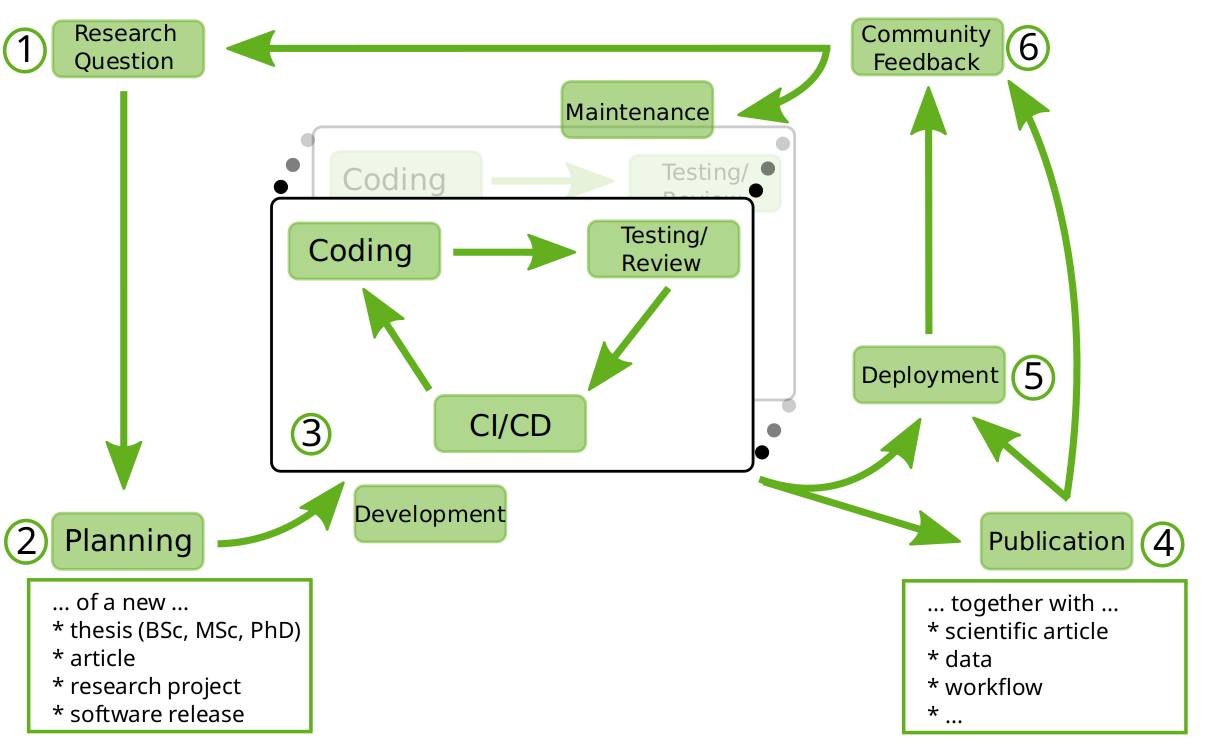
\includegraphics[width=0.99\linewidth]{imgs/rs_lifecycle.png}
    \caption{Research Software lifecycle.}
    \label{fig:rslifecycle}
\end{figure}

\subsection{Document organization}

The structure of the document is as follows. Section \ref{sec:classification} describes a survey conducted within the sub-group for articles and documents containing Quality Models and corresponding Quality Attributes as well as Quality Characteristics, while the attributes are listed in appendix \ref{appendix_qa}. In section \ref{sec:landscaping}, the RS stacks, RS types and user stories, are identified. This is deemed important because the recommendations in section \ref{sec:recommendations} for what Software Quality Attributes are more relevant depend on the stack, type and users in their role as developers. In section \ref{sec:perspectives}, the user perspectives are described, i.e., the point of view of developers, users and resource (or service) providers. In section \ref{sec:sw_in_prod}, recommendations are given for software release and management and services in production, while section \ref{sec:metadata} associates Quality Attributes and FAIR principles for RS. Last, in section \ref{sec:summary}, summary and conclusions are drawn.
